\documentclass[11pt]{article}

% load some asm stuff -
\usepackage{amssymb}
\usepackage{amsmath}
\usepackage{amsthm}
%\usepackage{palatino,lettrine}
\usepackage{fancyhdr}
\usepackage{epsfig}
\usepackage[square,sort,comma,numbers]{natbib}
\usepackage{simplemargins}
\usepackage{setspace}
\usepackage{wrapfig}
\usepackage{hyperref}
%\usepackage{boiboites}
\usepackage[margin=0pt,font=small,labelfont=bf]{caption}
\newcommand{\boldindex}[1]{\textbf{\hyperpage{#1}}}
\usepackage{makeidx}\makeindex
\bibliographystyle{plos2015}

\usepackage{algpseudocode}
\usepackage{algorithm}


% Set the size
%\textwidth = 6.75 in
%\textheight = 9.75 in
%\oddsidemargin = 0.0 in
%\evensidemargin = 0.0 in
%\topmargin = 0.01 in
%\headheight = 0.0 in
%\headsep = 0.25 in
%\parskip = 0.15in
% \doublespace
\setallmargins{1in}

\newtheorem{example}{Example}[section]
\newtheorem{thm}{Theorem}[section]
\newtheorem{property}{Property}[section]

\theoremstyle{definition}
\newtheorem{defn}[thm]{Definition}

\makeatletter
% \renewcommand\subsection{\@startsection
% 	{subsection}{2}{0mm}
% 	{-0.05in}
% 	{0.05\baselineskip}
% 	{\normalfont\normalsize\bfseries}}
\renewcommand\subsubsection{\@startsection
	{subsubsection}{2}{0mm}
	{-0.05in}
	{-0.5\baselineskip}
	{\normalfont\normalsize\itshape\bfseries}}
\renewcommand\paragraph{\@startsection
	{paragraph}{2}{0mm}
	{-0.05in}
	{-0.5\baselineskip}
	{\normalfont\normalsize\itshape}}
\makeatother
\linespread{1.1}

\fancypagestyle{proposal}{\fancyhf{}%
	\fancyhead[RO,LE]{\thepage}%
	\fancyhead[LO,RE]{CHEME 133 Module 4 Composite Contracts}%
	\renewcommand\headrulewidth{1pt}}
\pagestyle{proposal}

\usepackage{mdframed}
\definecolor{lgray}{rgb}{0.92,0.92,0.92}
\definecolor{antiquewhite}{rgb}{0.98,0.92,0.84}
\definecolor{lightskyblue}{rgb}{0.93,0.95,0.99}

% defn environment
\mdfdefinestyle{theoremstyle}{% 
    linecolor=black,linewidth=1pt,% 
    frametitlerule=true,% 
    frametitlebackgroundcolor=lgray, 
    innertopmargin=\topskip,} 
\mdtheorem[style=theoremstyle]{definition}{Definition}

% concept environment
\mdfdefinestyle{conceptstyle}{% 
    linecolor=black,linewidth=1pt,% 
    frametitlerule=true,% 
    frametitlebackgroundcolor=lightskyblue, 
    innertopmargin=\topskip,} 
\mdtheorem[style=conceptstyle]{concept}{Concept}
\newcommand{\newterm}[1]{{\it #1}}

% Single space'd bib -
\setlength\bibsep{0pt}

\renewcommand{\rmdefault}{phv}\renewcommand{\sfdefault}{phv}
%\newboxedtheorem[boxcolor=black, background=gray!5,titlebackground=orange!20,titleboxcolor = black]{color_box_example}{Example}{test}

% Change the number format in the ref list -
\renewcommand{\bibnumfmt}[1]{#1.}

% Change Figure to Fig.
\renewcommand{\figurename}{Fig.}
\usepackage{enumitem}
\setlist{noitemsep} % or \setlist{noitemsep} to leave space around whole list

%Joycelyn Chan, Joshua Lequieu, Michael Paull, Chidanand Balaji, Ryan Tasseff
%Our derivation follows closely the earlier development of Fredrickson \citep{Fredrickson:1976fk}.

% Begin ...
\begin{document}

%\begin{titlepage}
{\par\centering\textbf{\Large CHEME 133 Module 4: Analysis of American-Style Composite Options Contracts at Expiration}}
\vspace{0.2in}
{\par \centering \large{Jeffrey D. Varner}}
\vspace{0.05in}
{\par \centering \large{Smith School of Chemical and Biomolecular Engineering}}
{\par \centering \large{Cornell University, Ithaca NY 14853}}
% \vspace{0.1in}
% {\par \centering \small{Copyright \copyright\ Jeffrey Varner 2018. All Rights Reserved.}}\\

%\end{titlepage}
\date{}
\thispagestyle{empty}

\setcounter{page}{1}

\section*{Introduction}
Composite options contracts are financial instruments comprising two or more individual options contracts. 
The payoff and profit of a composite contract at expiration is the sum of the values of the individual contracts. 
The advantage of constructing composite contracts is that they can be used to construct complex payoffs and profit strategies 
from simple contract components. In this module, we will analyze composite contracts at expiration, 
where the composite contract comprises two or more American-style options.

\subsection*{General Formulation}
Call and put contracts can be combined to develop composite contract structures with interesting payoff diagrams. Let $\mathcal{C}$ be a composite contract with $d$ legs (individual contracts) where each leg is written for the same underlying asset \texttt{XYZ} and the same expiration date. 
Then, the payoff of the composite contract $\hat{V}(S(T),K_{1},\dots,K_{d})$ at time $T$ (expiration) is given by:
\begin{equation}
\hat{V}(S(T),K_{1},\dots,K_{d}) = \sum_{i\in\mathcal{C}}\theta_{i}\cdot{n_{i}}\cdot{V_{i}(S(T),K_{i}})
\end{equation}
where $K_{i}$ denotes the strike price of contract $i$, $\theta_{i}$ denotes the contract orientation $i$: $\theta_{i}=-1$ if contract $i$ is short (sold), 
otherwise $\theta_{i}=1$, and the quantity $n_{i}$ denotes the copy number of contract $i$.
The profit of the composite contract $\hat{P}$ at time $T$ (expiration) is given by:
\begin{equation}
\hat{P}(S(T),K_{1},\dots,K_{d}) = \sum_{i\in\mathcal{C}}\theta_{i}\cdot{n}_{i}\cdot{P}_{i}(S(T),K_{i})
\end{equation}
where $P_{i}(S(T),K_{i})$ denotes the profit of contract $i$. 
Finally, the profit for a contract of type $\star$ is given by:
\begin{equation}
P_{\star}(K,S(T)) = {V}_{\star}(K,S(T)) -  \mathcal{P}_{\star}(K,S(0))
\end{equation}
where $\mathcal{P}_{\star}(K,S(0))$ denotes the premium of contract $\star$, and ${V}_{\star}(K,S(T))$ 
denotes the payoff of contract $\star$ at expiration.

\section*{Defined-Risk Directional Composite Contracts}
Directional composite contracts make a directional assumption about the underlying asset's price movement and can be opened for a credit or debit.
A common directional composite contract is a \textit{spread}.

\subsection*{Put Vertical Spread}
A \texttt{put} vertical spread is constructed by combining 2 $\times$ \texttt{put} contracts; a short \texttt{put} contract generates income while a \texttt{long} put contract controls downside risk.  
Let contract $j$ have a strike price of $K_{j}$ and premium $\mathcal{P}_{j}$. 
The share price at expiration is given by $S$. 
Finally, let contract 1 be the short \texttt{put} leg $\theta_{1} = -1$ and contract 2 be the long \texttt{put} leg $\theta_{2} = 1$. 
Then, the profit for a single \texttt{put} vertical spread at expiration is given by:
\begin{equation}
\hat{P} = -P_{1}+P_{2}
\end{equation}
which, after substitution of the profit functions for a put contract, gives:
\begin{equation}
\hat{P} = \left(K_{2} - S\right)^{+} - \left(K_{1} - S\right)^{+} + \left(\mathcal{P}_{1} - \mathcal{P}_{2}\right)
\end{equation}
where $V_{p} = (K-S)^{+}=\max(K-S,0)$ is the payoff function for a \texttt{put} contract. 
The first term is the net payout of the two legs of the spread, while the second term is the net cost of the two contracts. 
The maximum possible profit, loss, and breakeven conditions are given by:
\begin{itemize}
\item{The maximum possible profit of $\left(\mathcal{P}_{1} - \mathcal{P}_{2}\right)$ will occur when $S\geq{K_{1}}$.}
\item{The maximum possible loss of $K_{2} - K_{1} + \left(\mathcal{P}_{1} - \mathcal{P}_{2}\right)$ will occur when $S\leq{K_{2}}$.}
\item{The vertical put spread will breakeven when $S =  K_{1}+\left(\mathcal{P}_{2} - \mathcal{P}_{1}\right)$.}
\end{itemize}

\subsection*{Bearish call credit spread}
A bear \texttt{call} credit spread is an options strategy used 
when a trader expects a decline in the price of the underlying asset. 
Assume the initial share price of the underlying asset is $S_{o}$ (when we are opening the trade).
For this trade, we sell a \texttt{call} contract at $K_{1}<S_{o}$ for $\mathcal{P}_{1}$, 
and buy a \texttt{call} contract at $K_{2}>S_{o}$ for $\mathcal{P}_{2}$. The profit function 
for the bear \texttt{call} credit spread is given by:
\begin{equation}
\hat{P} = (S-K_{2})^{+} - (S-K_{1})^{+} + (\mathcal{P}_{1}-\mathcal{P}_{2})
\end{equation}
where $V_{c} = (S-K)^{+}=\max(S-K,0)$ is the payoff function for a \texttt{call} contract. 
The first two terms are the net payout of the two legs of the spread, while the last term is the net cost of the two contracts. 
The maximum possible profit, loss, and breakeven conditions are given by:
\begin{itemize}
\item{The maximum possible profit of $\left(\mathcal{P}_{1} - \mathcal{P}_{2}\right)$ will occur when $S\leq{K_{1}}$.}
\item{The maximum possible loss of $\left(\mathcal{P}_{1} - \mathcal{P}_{2}\right) -(K_{2} - K_{1})$ will occur when $S\geq{K_{2}}$.}
\item{The bear \texttt{call} spread will breakeven when $S =  K_{1}+\left(\mathcal{P}_{1} - \mathcal{P}_{2}\right)$.}
\end{itemize}

\section*{Neutral Composite Contracts}
Neutral composite contracts make no directional assumption about the price movement of the underlying asset and can be opened for credit or debit.
Two common directional composite contracts are the \textit{straddle} and the \textit{strangle}.	

\subsection*{Straddles}
A \href{https://www.investopedia.com/terms/s/straddle.asp}{straddle} is a neutral strategy constructed by simultaneously buying (or selling) 
a put and a call option on the same underlying asset \texttt{XYZ}, with the same expiration and the same strike price (Fig. \ref{fig:options-short-straddle-profit}). 

\begin{figure}[h]
    \centering
    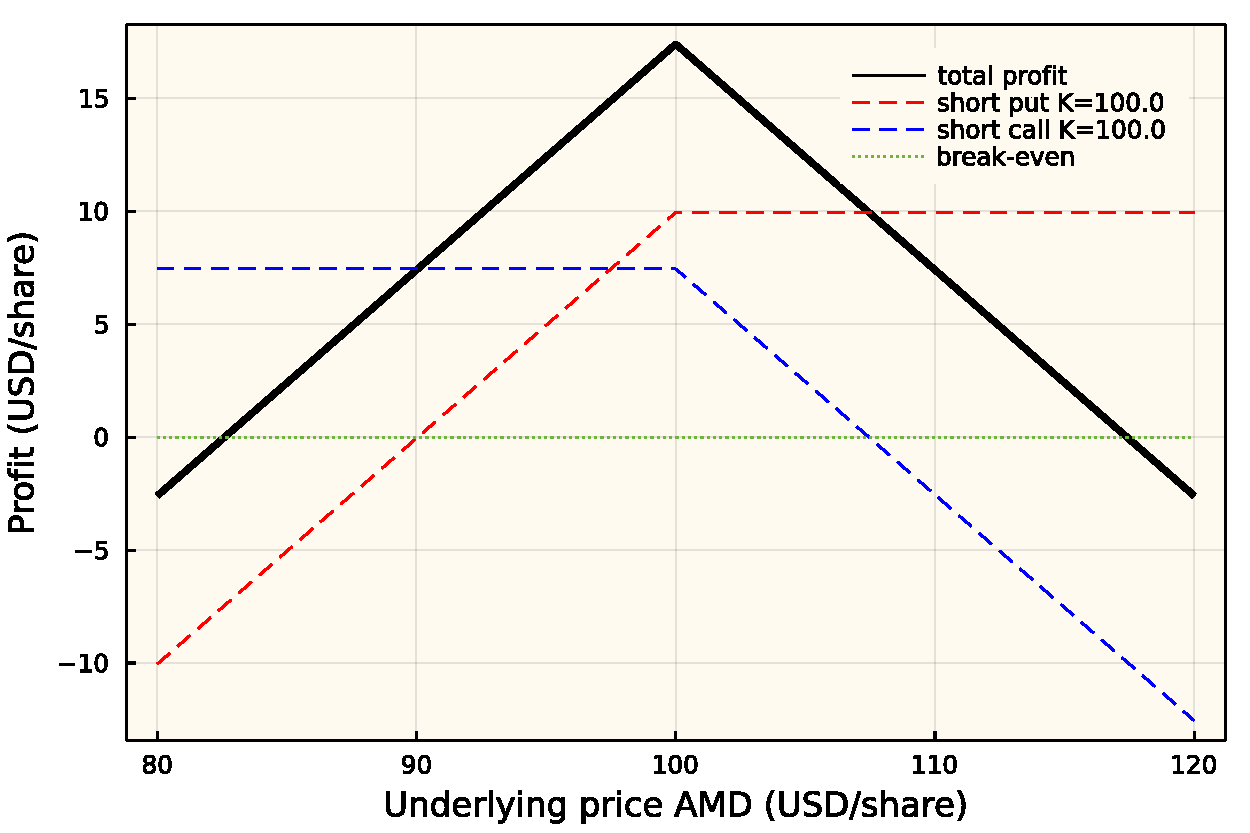
\includegraphics[width=0.75\textwidth]{./figs/Fig-AMD-Profit-Short-Straddle.pdf}
    \caption{Schematic of the profit for a short straddle trade written for Advanced Micro Devices, Inc. with ticker symbol \texttt{AMD}.
	A short straddle is a neutral strategy constructed by simultaneously selling a put and a call option on the same underlying asset \texttt{AMD}, with the same expiration and strike price.
	Conversely, a long straddle is a neutral strategy constructed by simultaneously buying a put and a call option on the same underlying asset \texttt{AMD}, with the same expiration and strike price.
	A long straddle has the same breakeven points as a short straddle, but the profit and loss are reversed, i.e., the profit diagram is rotated around the breakeven line.
	Thus, a long straddle has a defined maximum loss and an unlimited maximum possible profit.
	}\label{fig:options-short-straddle-profit}
\end{figure}

Depending upon the choice of the strike prices and whether an investor buys or sells both legs, 
a \href{https://www.investopedia.com/terms/s/straddle.asp}{straddle} can be initiated as a credit or debit and potentially have undefined profit or loss.
Let $K_{j}$ denote the strike price of contract $j$ (USD/share), where the price of contract $j$ is $\mathcal{P}_{j}$ (USD/share). 
Further, let index $j=1$ denote the \texttt{put} contract, $j=2$ denote the \texttt{call} contract; 
for a straddle $K_{1}= K_{2}\equiv{K}$ (both legs have the same strike). The profit for a single straddle contract $\hat{P}$ at expiration is given by:
\begin{equation}
\hat{P} = \theta\cdot\left(P_{1}+P_{2}\right)
\end{equation}
where $\theta_{1}=\theta_{2}\equiv\theta$ denotes a direction parameter: $\theta=-1$ if each leg is sold (short),
$\theta=1$ otherwise. After substitution of the profit functions for a \texttt{put} and a \texttt{call} contract, the overall profit $\hat{P}$ for a \texttt{straddle} 
is given by:
\begin{equation}
\hat{P} = \theta\cdot\Bigl[(K-S)^{+}+(S-K)^{+}-(\mathcal{P}_{1}+\mathcal{P}_{2})\Bigr]
\end{equation}
where $V_{p} = (K-S)^{+}=\max(K-S,0)$ is the payoff function for the \texttt{put} contract, and $V_{c} = (S-K)^{+} = \max(S-K,0)$ is the payoff function for the \texttt{call} contract. 
The profit (or loss) of a straddle has three regimes given by:
\begin{equation}
\hat{P} = \begin{cases}
  \theta\cdot\Bigl[(S(T)-K)-\left(\mathcal{P}_{1}+\mathcal{P}_{2}\right)\Bigr]  & S(T)>K \\
  -\theta\cdot\Bigl[\mathcal{P}_{1}+\mathcal{P}_{2}\Bigr] & S(T)=K \\
    \theta\cdot\Bigl[(K-S(T))-\left(\mathcal{P}_{1}+\mathcal{P}_{2}\right)\Bigr] & S(T)<K
\end{cases}
\end{equation}
where $S(T)$ denotes the share price of the underlying asset at expiration. Finally, a straddle has two possible breakeven points denoted as $S^{+}$ and $S^{-}$:
\begin{equation}
	\mathcal{B}(T) = \begin{cases}
		S^{+} = K + \left(\mathcal{P}_{1}+\mathcal{P}_{2}\right) & S(T)>K \\
		S^{-} = K - \left(\mathcal{P}_{1}+\mathcal{P}_{2}\right) & S(T)<K
	\end{cases}
\end{equation}
where $S^{+}$ denotes the upper breakeven point, and $S^{-}$ denotes the lower breakeven point.

\subsection*{Strangles}
A \href{https://www.investopedia.com/terms/s/strangle.asp}{strangle} is a neutral strategy constructed by simultaneously buying (or selling)
a \texttt{put} and a \texttt{call} option on the same underlying asset \texttt{XYZ}, with the same expiration, but with different strike prices (Fig. \ref{fig:options-short-strangle-profit}).

\begin{figure}[h]
    \centering
    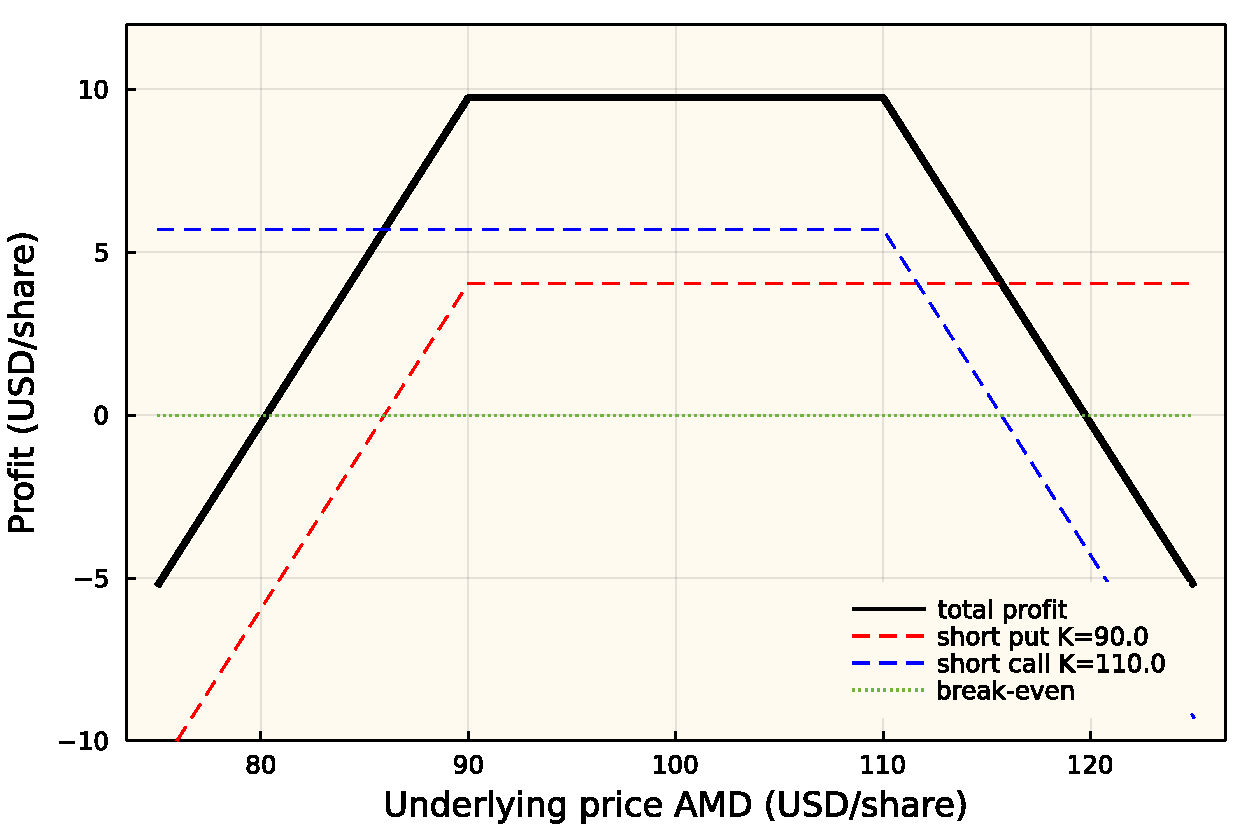
\includegraphics[width=0.75\textwidth]{./figs/Fig-AMD-Profit-Short-Strangle.pdf}
    \caption{Schematic of the profit for a short strangle trade written for Advanced Micro Devices, Inc. with ticker symbol \texttt{AMD}.
	A short strangle is a neutral, undefined risk strategy constructed by simultaneously selling a put and a call option on the same underlying asset \texttt{AMD}, with the same expiration but different strike prices.
	On the other hand, a long strangle is a neutral strategy constructed by simultaneously buying a put and a call option on the same underlying asset \texttt{AMD}, with the same expiration but different strike prices.
	A long strangle has the same breakeven points as a short strangle, but the profit and loss are reversed, i.e., the profit diagram is rotated around the breakeven line.
	Thus, a long strangle has a defined maximum loss and an undefined maximum possible profit.
	}\label{fig:options-short-strangle-profit}
\end{figure}

Depending upon the choice of the strike prices and whether an investor buys or sells both legs, a \href{https://www.investopedia.com/terms/s/strangle.asp}{strangle} 
can be initiated for a credit or debit and potentially have undefined profit or loss. Let $K_{j}$ denote the strike price of contract $j$ (USD/share), 
where the price of contract $j$ is $\mathcal{P}_{j}$ (USD/share). Further, let index $j=1$ denote the \texttt{put} contract, $j=2$ denote the \texttt{call} contract; 
for a strangle $K_{1}<K_{2}$. The profit for a single strangle contract $\hat{P}$ at expiration is given by:
\begin{equation}
\hat{P} = \theta\cdot\left(P_{1}+P_{2}\right)
\end{equation}
where $\theta_{1} = \theta_{2}\equiv\theta$ denotes a direction parameter: $\theta=-1$ if each leg is sold (short), $\theta=1$ otherwise. 
After substitution of the profit functions for a \texttt{put} and a \texttt{call} contract, the overall profit $\hat{P}$ for a \texttt{strangle} 
is given by:
\begin{equation}
\hat{P} = \theta\cdot\Bigl[(K_{1}-S)^{+}+(S-K_{2})^{+}-(\mathcal{P}_{1}+\mathcal{P}_{2})\Bigr]
\end{equation}
where $V_{p} = (K_{1}-S)^{+}=\max(K_{1}-S,0)$ is the payoff for the \texttt{put} contract, 
and $V_{c} = (S-K_{2})^{+} = \max(S-K_{2},0)$ is the payoff for the \texttt{call} contract. 
The profit (or loss) of a strangle has three regimes given by:
\begin{equation}
\hat{P} = \begin{cases}
  \theta\cdot\Bigl[(S(T)-K_{2})-\left(\mathcal{P}_{1}+\mathcal{P}_{2}\right)\Bigr]  & S(T)>K_{2} \\
  -\theta\cdot\Bigl[\mathcal{P}_{1}+\mathcal{P}_{2}\Bigr] & K_{1}\leq{S(T)}\leq{K_{2}} \\
  \theta\cdot\Bigl[(K_{1}-S(T))-\left(\mathcal{P}_{1}+\mathcal{P}_{2}\right)\Bigr] & S(T)<{K_{1}}
\end{cases}
\end{equation}
where $S(T)$ denotes the share price of the underlying asset at expiration. 
Finally, a strangle has two possible breakeven points denoted as $S^{+}$ and $S^{-}$:
\begin{equation}
	\mathcal{B}(T) = \begin{cases}
		S^{+} = K_{1} - \left(\mathcal{P}_{1}+\mathcal{P}_{2}\right) & S(T) > K_{2} \\
		S^{-} = K_{2} + \left(\mathcal{P}_{1}+\mathcal{P}_{2}\right) & S(T) < K_{1}
	\end{cases}
\end{equation}
where $S^{+}$ denotes the upper breakeven point, and $S^{-}$ denotes the lower breakeven point.

\subsection*{Iron Condor}
Iron Condors are examples of defined-risk neutral strategies, i.e., they make no directional assumption about the price movement of the underlying asset, 
and can be opened for credit or debit.
However, unlike straddles and strangles, iron condors have a defined maximum loss and maximum possible profit (Fig. \ref{fig:options-iron-condor-profit}).
An \href{https://www.investopedia.com/terms/i/ironcondor.asp}{iron condor} is a neutral defined risk position constructed 
by \textit{selling} a put (1) and call (2) options on the underlying asset \texttt{XYZ}, 
while simultaneously \textit{buying} a put (3) and call (4) options on \texttt{XYZ}. 
All the legs of an \href{https://www.investopedia.com/terms/i/ironcondor.asp}{iron condor} have the same underlying asset \texttt{XYZ}, 
and have the same expiration, but they have different strike prices where $K_{3}<K_{1}<K_{2}<K_{4}$. 
In particular, the two short options are sold with strikes on either side of the current share price $S_{o}$ of \texttt{XYZ}, 
with the short put strike price $K_{1}<S_{o}$ and the short call strike price $K_{2}>S_{o}$. 
Then, the long legs are purchased above and below the short strikes.  
Thus, an \href{https://www.investopedia.com/terms/i/ironcondor.asp}{iron condor} position has the character of a 
\href{https://www.investopedia.com/terms/s/strangle.asp}{strangle} combined with a vertical spread. 

\begin{figure}[h]
    \centering
    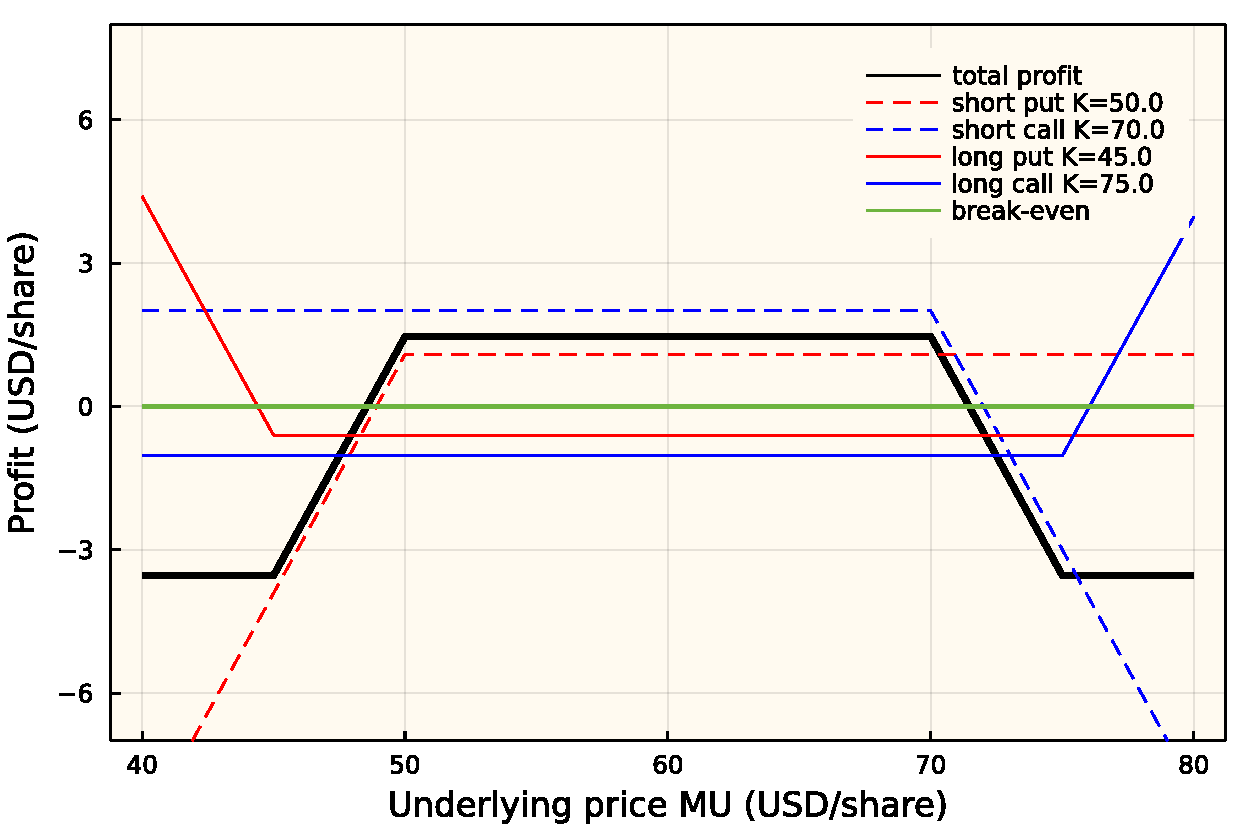
\includegraphics[width=0.75\textwidth]{./figs/Fig-MU-Profit-IronCondor.pdf}
    \caption{Schematic of the profit for an Iron Condor on Micron Technologies with ticker symbol \texttt{MU}.
	An iron condor is a neutral defined risk position constructed by selling a put and call options on the underlying asset \texttt{MU},
	while simultaneously buying a put and call options on \texttt{MU}. Thus, the maximum possible profit and loss are defined when the trade is opened.
	}\label{fig:options-iron-condor-profit}
\end{figure}

Let the current share price of \texttt{XYZ} be $S_{o}$ USD/share, and let $S(T)$ denote the share price of \texttt{XYZ} at expiration. 
Further, let $K_{j}$ denote the strike price of contract $j$ (USD/share), where the price of contract $j$ is $\mathcal{P}_{j}$ (USD/share). 
Finally, let index $j=1$ denote the short put contract, $j=2$ denote the short call contract,  $j=3$ denote the long put contract and  $j=4$ denote the long call contract; 
for an \href{https://www.investopedia.com/terms/i/ironcondor.asp}{iron condor} $K_{3} < K_{1} <K_{2} < K_{3}$. 
Then, the profit for a single iron condor contract $\hat{P}$ at expiration is given by:
\begin{equation}
\hat{P} = \theta_{1}P_{1} + \theta_{2}P_{2} + \theta_{3}P_{3} + \theta_{4}P_{4}
\end{equation}
where $\theta_{1}=\theta_{2} = -1$ (short legs) and $\theta_{3}=\theta_{4} = 1$ (long legs). 
After substitution of the profit functions for put and call contracts, the overall profit $\hat{P}$ is given by:
\begin{equation}
\hat{P} = -(K_{1}-S)^{+} - (S-K_{2})^{+} + (K_{3} - S)^{+} + (S-K_{4})^{+} + \left(\mathcal{P}_{1} + \mathcal{P}_{2} - \mathcal{P}_{3}-\mathcal{P}_{4}\right)
\end{equation}
where $(K_{\star}-S)^{+}=\max(K_{\star}-S,0)$ and $(S-K_{\star})^{+} = \max(S-K_{\star},0)$. 
The profit (or loss) of an iron condor has several important regimes given by:
\begin{equation}
\hat{P} = \begin{cases}
  K_{2} - K_{4} + \Bigl(\mathcal{P}_{1} + \mathcal{P}_{2} - \mathcal{P}_{3}-\mathcal{P}_{4}\Bigr)  & S>K_{4} \\
  K_{2} - S + \Bigl(\mathcal{P}_{1} + \mathcal{P}_{2} - \mathcal{P}_{3}-\mathcal{P}_{4}\Bigr)  & K_{2}<S<K_{4} \\
  \Bigl(\mathcal{P}_{1} + \mathcal{P}_{2} - \mathcal{P}_{3}-\mathcal{P}_{4}\Bigr) & K_{1}\leq{S}\leq{K_{2}} \\
  S - K_{1} + \Bigl(\mathcal{P}_{1} + \mathcal{P}_{2} - \mathcal{P}_{3}-\mathcal{P}_{4}\Bigr) & K_{3}<S<K_{1} \\
  K_{3} - K_{1} + \Bigl(\mathcal{P}_{1} + \mathcal{P}_{2} - \mathcal{P}_{3}-\mathcal{P}_{4}\Bigr) & S<K_{3}
\end{cases}
\end{equation}
Finally, an iron condor has two possible breakeven points denoted as $S^{+}$ and $S^{-}$:
An \href{https://www.investopedia.com/terms/i/ironcondor.asp}{iron condor} has two break-even points $S^{+}$ and $S^{-}$ 
where we know that $K_{2}<S^{+}<K_{4}$ and $K_{3}<S^{-}<K_{1}$. Thus, the low break-even point $S^{-}$ is given by:
\begin{equation}
S^{-} = K_{1} - \Bigl(\mathcal{P}_{1} + \mathcal{P}_{2} - \mathcal{P}_{3}-\mathcal{P}_{4}\Bigr)
\end{equation}
while the high break-even point $S^{+}$ is given by:
\begin{equation}
S^{+} = K_{2} + \Bigl(\mathcal{P}_{1} + \mathcal{P}_{2} - \mathcal{P}_{3}-\mathcal{P}_{4}\Bigr)
\end{equation}

\section*{Summary}
In this module, we have analyzed the profit and loss of American-style composite contracts at expiration.
We considered two types of composite contracts: directional and neutral.
Directional composite contracts make a directional assumption about the underlying asset's price movement, which can be opened for credit or debit.
Directional composite contracts, such as put vertical spreads and bearish call credit spreads, are examples of a defined-risk directional strategy.
On the other hand, neutral composite contracts make no directional assumption about the underlying asset's price movement and can be opened for a credit or debit.
These include straddles and strangles, examples of undefined profit or loss strategies, and Iron Condors, an example of defined-risk neutral strategies.

% \bibliography{References_v1}

\clearpage
\printindex

\end{document}
